\section{Titulo}
contenido bla bla bla.

\begin{lstlisting}[style=JavaScriptStyle, caption={Código JavaScript}]
// comentario
var valor = 5;
console.log(valor);
\end{lstlisting}

\subsection{Subtitulo}
contenido bla bla bla.

\begin{figure}[h]
\centering
\fbox{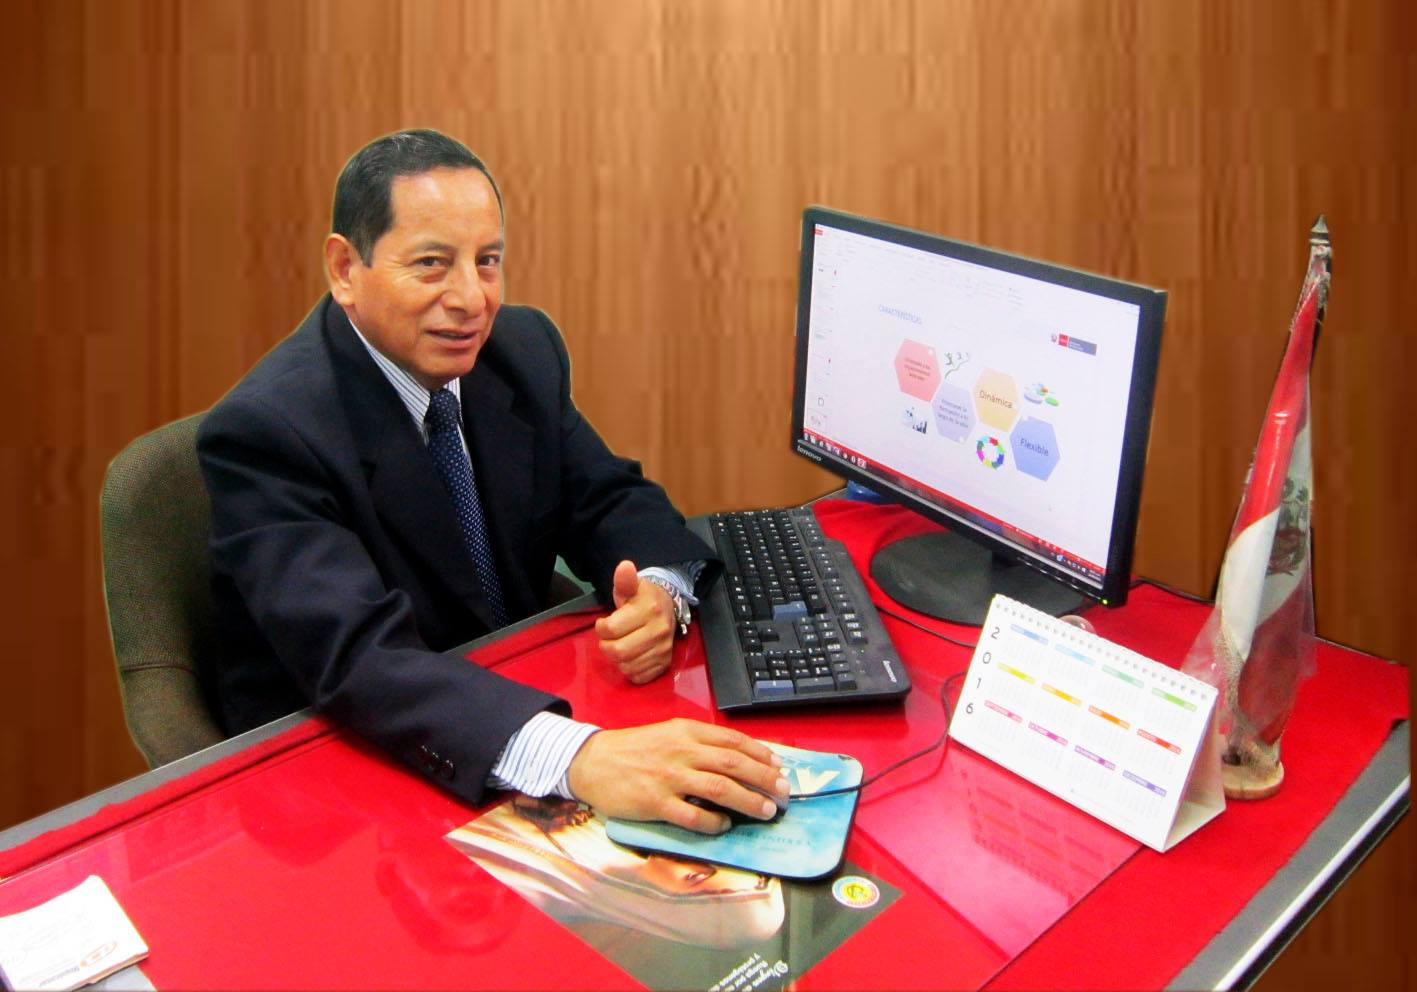
\includegraphics[width=0.8\textwidth]{img/beltran.png}}
\caption{Descripción de la imagen}
\end{figure}

\subsubsection{Sub Subtitulo}

\begin{table}[H]
\caption{Descripción de la tabla}
\resizebox{\textwidth}{!}{ % Escala la tabla a todo el ancho de la página
\begin{tabular}{|p{3.1cm}|p{6.5cm}|} %|c|c| %|l|l|
\hline
\textbf{Objeto} & \textbf{Color}\\ \hline
mouse & negro
\\ \hline

teclado & blanco
\\ \hline
\end{tabular}
}
\end{table}
